Assume the agent interacts with a simple two-state MDP shown below. Every episode begins in state $X$, and ends when the agent transitions from state $Y$ to the terminal state (denoted by gray box). Let's denote the set of states as $\mathcal{S} = \{X,Y\}$. There is only one possible action in each state, so there is only one possible policy in this MDP. Let's denote the set of actions $\mathcal{A} = \{A\}$. In state $Y$ the agent terminates when it takes action $A$ and sometimes gets a reward of +1000, and sometimes gets a reward of -1000: the reward on this last transition is stochastic. Let $\gamma = 1.0$. 
\begin{figure}[h!]
  \center
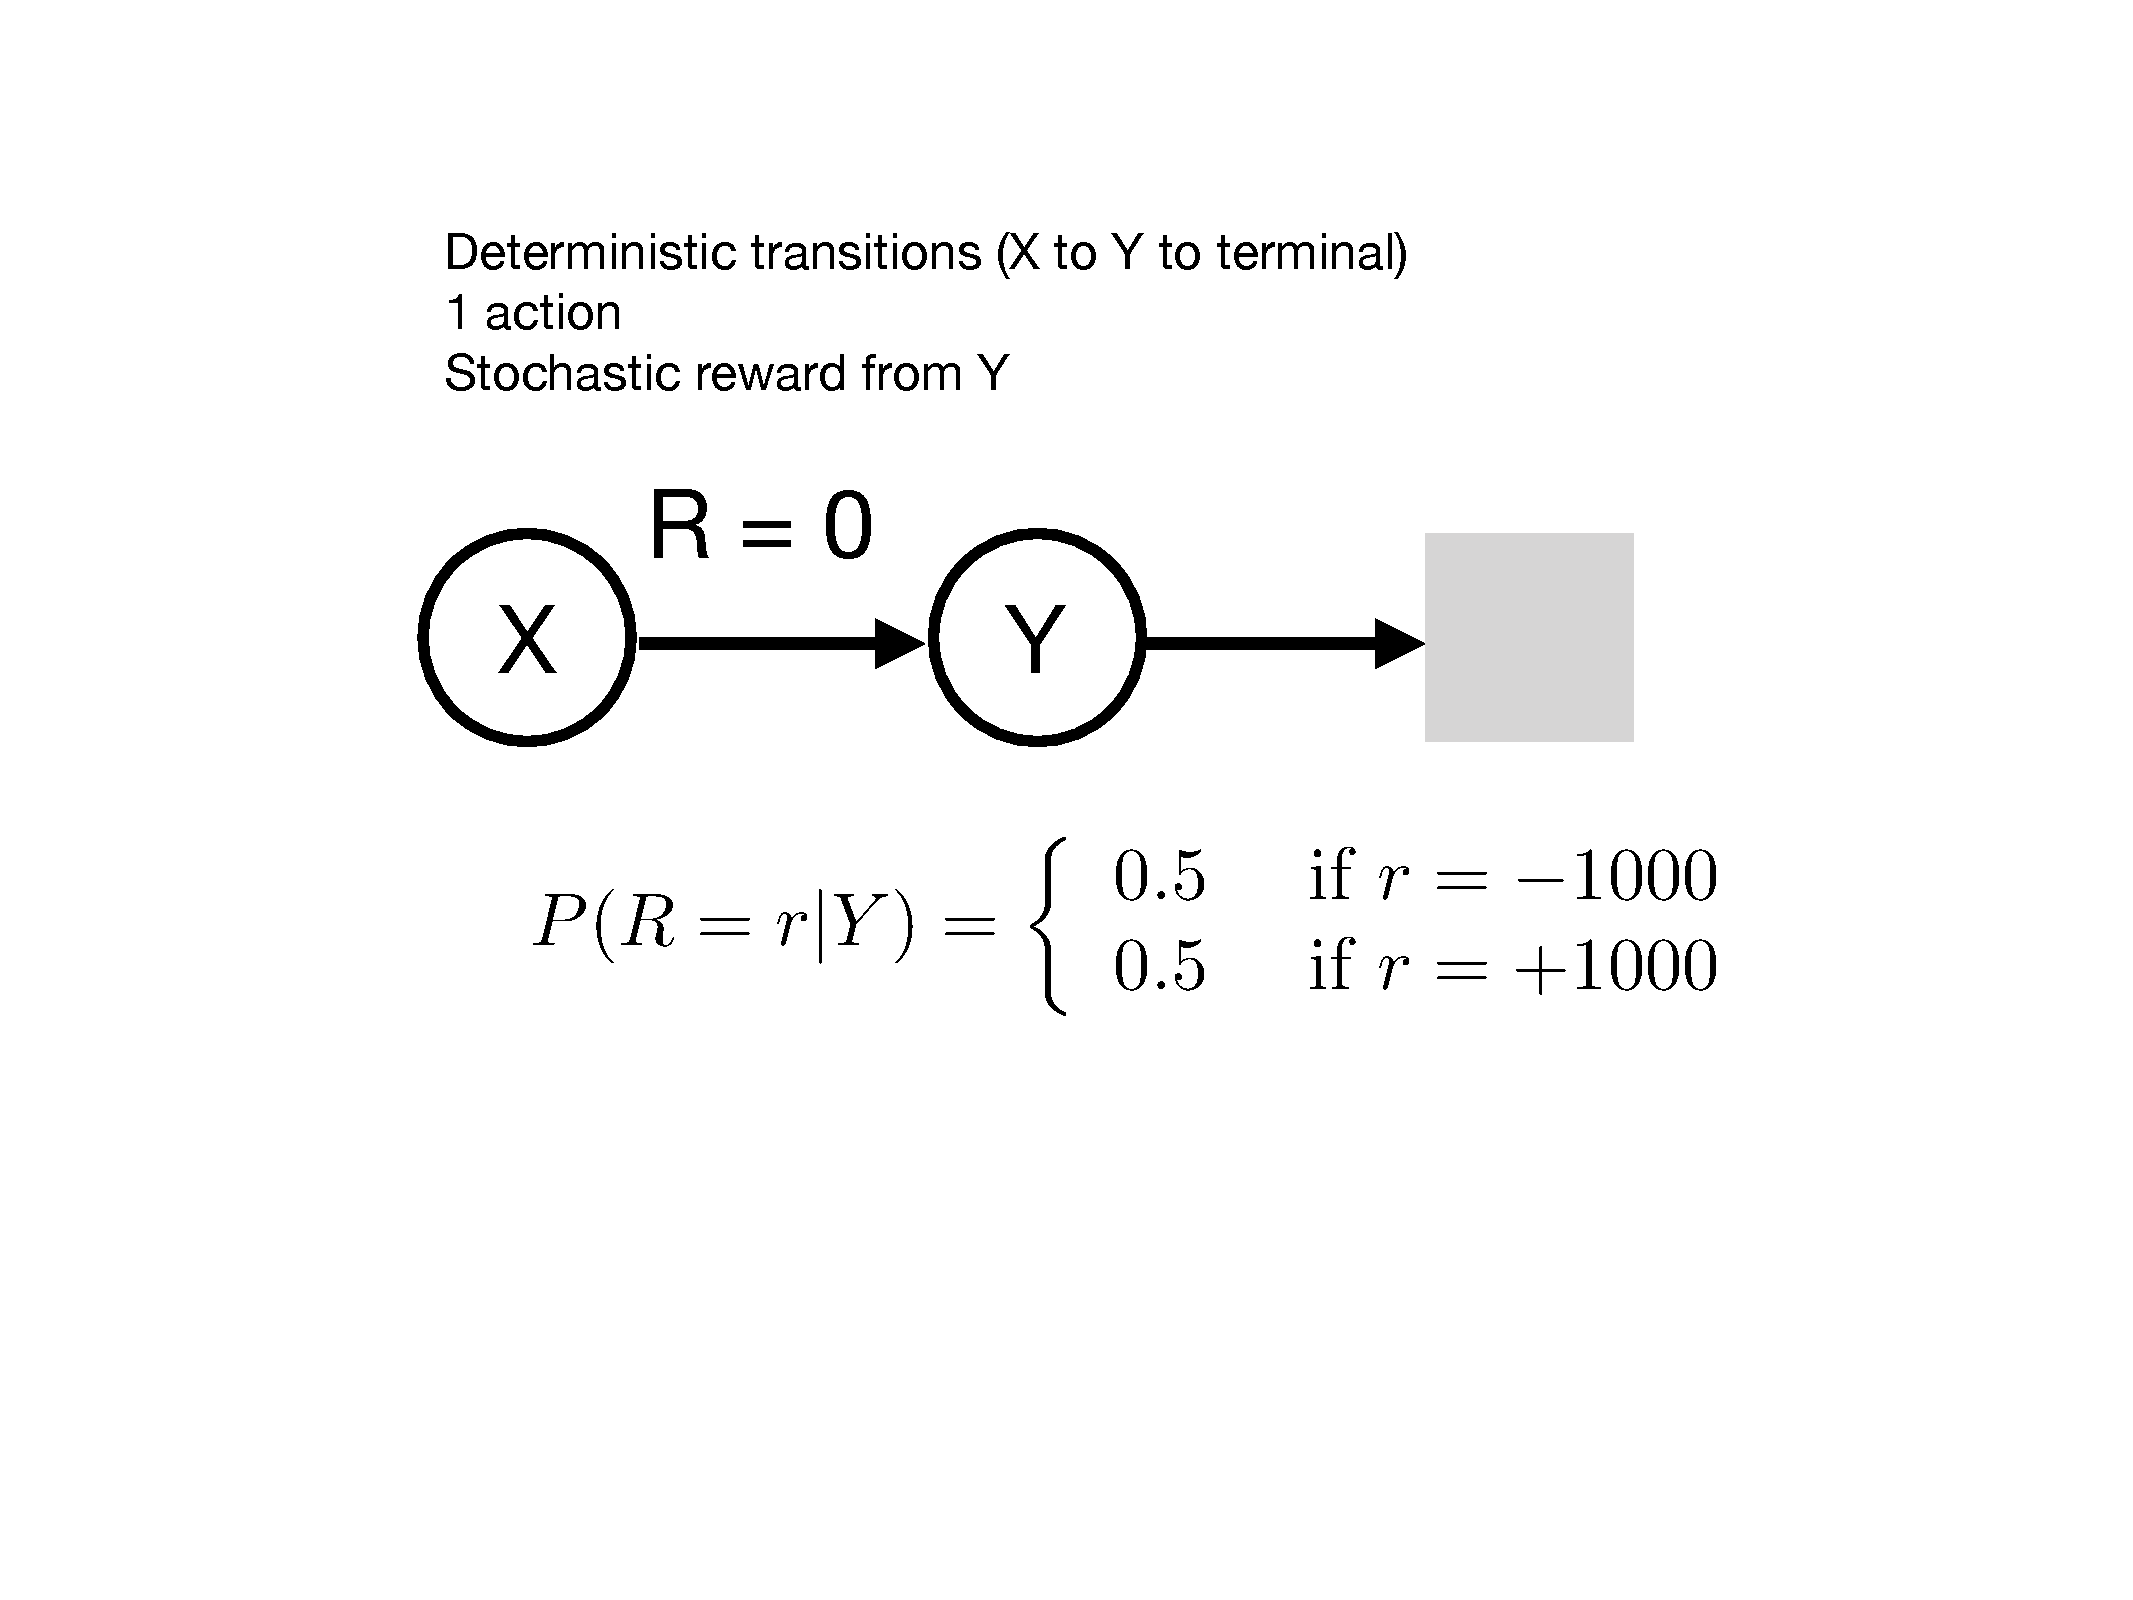
\includegraphics[width=0.5\linewidth]{figures/c2m2_xy.pdf}
\end{figure}
%
\begin{enumerate}
%
\item Write down $\pi(a|s) ~\forall~ s\in\mathcal{S}, a\in\mathcal{A}$.
\item Write down all the possible trajectories (sequence of states, actions, and rewards) in this MDP that start from state $X$?
\item What is the value of policy $\pi$ (i.e. what is $v_\pi(X), v_\pi(Y)$)?
\item Assume our estimate is equal to the value of $\pi$. That is $V(s) = v_\pi(s) ~\forall~ s\in\mathcal{S}$. Now compute the TD-error $\delta_t = R_{t+1} + \gamma V(S_{t+1}) - V(S_t)$ for the transition from state $Y$ to the terminal state, assuming $R_{t+1} = +1000$. Why is the TD-error not zero if we start with $V(Y) = v_\pi(Y)$?
\item Based on your answer to (d), what does this mean for the TD-update, for constant $\alpha = 0.1$? Will $V(Y) = v_\pi(Y) = 0$ after we update the value using TD? Recall the TD-update is $V(S_t) \gets V(S_t) + \alpha \delta_t$.  
\item What is the expected TD-update---the update on average---from state $Y$ for a given $V$?
\item Assume again that $V=v_\pi$. What is the expectation and the variance of the TD update from state $X$? What is the expectation and the variance of the Monte-carlo update from state $X$?
\end{enumerate}

%% \textbf{Answer:}
%% \begin{enumerate}
%% \item $\pi(A|X) = 1$ and $\pi(A|Y) = 1$.
%% \item $(S_0=X, A_0=A, R_1=0, S_1=Y, A_1=A, R_2=1000, S_2=T)$ and $(S_0=X, A_0=A, R_1=0, S_1=Y, A_1=A, R_2=-1000, S_2=T)$.
%% \item We know that $v_\pi(S) = \sum_a \pi(a|s) \sum_{s', r} p(s', r | s, a) [r + \gamma v_\pi(s')]$ and that $v_\pi(T) \doteq 0$. Using this $v_\pi(Y) = 1\cdot[0.5 (1000 + \gamma v_\pi(T)) + 0.5 (-1000 + \gamma v_\pi(T))] = 0$ and $v_\pi(X) = 1 \cdot 1 \cdot [0 + \gamma v_\pi(Y)] = 0$.
%% \item $\delta_t = R_{t+1} + \gamma v_\pi(S_{t+1}) - v_\pi(S_t) = 1000 + \gamma v_\pi(T) - v_\pi(Y) = 1000$. The TD error is zero in expectation for the true value function, i.e. $\E[\delta_t | S_t] = 0$ for $v_\pi$ as we later show. Its value doesn't have to be zero.
%% \item Based on the above sub--question, if we make the TD update for state $Y$ using $\alpha=0.1$, we would obtain: $V(Y) = V(Y) + 0.1 \times 1000 = 100$. If we continue to make such updates, we can see that $V(Y)$ will oscillate without ever going to zero.
%% \item $\E[\delta_t | S_t] = \sum_{r} p(r | Y) (r + \gamma v_\pi(T) - v_\pi(Y)) = 0.5 (1000 + \gamma v_\pi(T) - v_\pi(Y)) + 0.5 (-1000 + \gamma v_\pi(T) - v_\pi(Y)) = 0$.
%% \item
%%   \textbf{TD update:} \textcolor{red}{I'm not sure about this.} The expectation of the TD update is
%%    \begin{equation*}
%%     \E[\delta | X] = \E[0 + \gamma v_\pi(Y) - v_\pi(X) | X] = 0,
%%   \end{equation*}
%%    since each $v_\pi(X) =  v_\pi(Y)  = 0$.
%%    The variance of the TD update is
%%    \begin{IEEEeqnarray*}{lCl}
%%       \V[\delta | X] &=& \E[\delta^2 | X] - \E[\delta | X]^2\\
%%       &=& \E[(0 + \gamma v_\pi(Y) - v_\pi(X))^2 | X] \\
%%       &=& 0.
%%     \end{IEEEeqnarray*}
%%   \textbf{MC update:} The expectation of the MC update is
%%   \begin{equation*}
%%     \E[G - v_\pi(X) | X] = 0.5 \times1000 + 0.5 \times(-1000) = 0.
%%   \end{equation*}

%%   Similarly, the variance is
%%     \begin{IEEEeqnarray*}{lCl}
%%       \V[G - v_\pi(X) | X] &=& \E[(G - v_\pi(X))^2 | X] - \E[G - v_\pi(X) | X]^2\\
%%       &=& \E[(G - v_\pi(X))^2 | X] \\
%%       &=& 0.5 \times1000^2 + 0.5 \times(-1000)^2 \\
%%       &=& 1000^2.
%%     \end{IEEEeqnarray*}
%% \end{enumerate}
